% easychair.tex,v 3.5 2017/03/15

\documentclass[a4paper]{easychair}

\usepackage{doc}

% use this if you have a long article and want to create an index
% \usepackage{makeidx}

% In order to save space or manage large tables or figures in a
% landcape-like text, you can use the rotating and pdflscape
% packages. Uncomment the desired from the below.
%
% \usepackage{rotating}
% \usepackage{pdflscape}

%\makeindex

%% Front Matter
%%
% Regular title as in the article class.
%
\title{Towards heterogeneous behavioral model composition}

% Authors are joined by \and. Their affiliations are given by \inst, which indexes
% into the list defined using \institute
%
\author{
Tim Kräuter
\and
Adrian Rutle
\and
Yngve Lamo
}

% Institutes for affiliations are also joined by \and,
\institute{
  Høgskulen på Vestlandet\\
  Bergen, Norway\\
  \email{tkra@hvl.no, aru@hvl.no, yla@hvl.no}
 }

%  \authorrunning{} has to be set for the shorter version of the authors' names;
% otherwise a warning will be rendered in the running heads. When processed by
% EasyChair, this command is mandatory: a document without \authorrunning
% will be rejected by EasyChair

\authorrunning{T. Kräuter et al.}

% \titlerunning{} has to be set to either the main title or its shorter
% version for the running heads. When processed by
% EasyChair, this command is mandatory: a document without \titlerunning
% will be rejected by EasyChair
\titlerunning{Heterogeneous behavioral model composition}

\usepackage{glossaries}

\newacronym{mde}{MDE}{Model-driven engineering}
\newacronym[
    shortplural={GGs},
    longplural={graph grammars}
]{gg}{GG}{graph grammar}
\newacronym{bpmn}{BPMN}{Business Process Modeling Notation}
\newacronym{ct}{CT}{category theory}
\newacronym{uml}{UML}{Unified Modeling Language}
\newacronym{dsl}{DSL}{Domain Specific Language}
\newacronym{csp}{CSP}{Communication Sequential Processes}

\begin{document}

\maketitle
% 2-3 pages abstract wanted by NWPT

%------------------------------------------------------------------------------
\section{Introduction}
% Introduction/Motivation
A common approach to handle the increasing complexity of software systems is \gls*{mde}.
\gls*{mde} envisions a clear separation of concerns by modeling each aspect of a system separately \cite{franceModeldrivenDevelopmentComplex2007}.
However, these individual models must be composed to execute the system or reason about global properties \cite{kienzleUnifyingFrameworkHomogeneous2019}.

% Narrowing down
Our contribution addresses the problem of how the individual models can be composed to describe the entire software system, even if the used models are heterogeneous, i.e., do not conform to the same modeling language.
In particular, we address the composition of behavioral models since its structural counterpart has been the focus of a significant amount of research already, for example, in \cite{kienzleUnifyingFrameworkHomogeneous2019, klareCommonalitiesPreservingConsistency2019, stunkelComprehensiveSystemsFormal2021}.
We further limit the behavioral models to those describing discrete behavior such as finite state machines, \gls*{bpmn} diagrams, process algebras, and Petri nets. % Untimed variants and only a subset of BPMN.

% Summary of the results/contribution
Our contribution can be summarized as follows.
Given a collection of behavioral models describing one system coordinated using our two types of interactions, we can construct a model representing the system's behavior.
One can then analyze the state space generated by the composite model to reason about global properties and analyze possible execution paths of the system.
We will use \glspl*{gg} as an underlying formalism to explain our approach in this contribution.
However, one could also choose a different formalism if it supports our two types of interactions and generates a global state space.
This contribution extends our work in \cite{krauterBehavioralConsistencyHeterogeneous2021} by adding asynchronous communication and an example showing how to implement hierarchical composition.

An approach with similar goals uses event structures as an underlying formalism and event scheduling to model behavioral relations \cite{kienzleUnifyingFrameworkHomogeneous2019}.
However, it is only applied to compose homogeneous models and does not include model-checking.

\section{Heterogeneous behavioral model composition}
We assume that each behavioral model describes a component of the overall system running independently and in parallel when it is not interacting with other components.
Each component, i.e., behavioral model, should interact at least once with a different model to contribute to the composite system behavior.

% We suggest 2 primitives to relate behavioral models: synchronous and asynchronous communication (currently without data).
Our approach supports two types of interactions between behavioral models: \textit{synchronous} and \textit{asynchronous} communication.
One can use synchronous communication to model that one component acquires a resource realized in a separate model since it is shared across the entire system.
Asynchronous communication can, for example, be used to model that two components communicate using a messaging system or by writing/consuming files in a shared file system.
Defining synchronous communication leads to two components becoming active simultaneously, while asynchronous communication only requires one component to be active. 

Our model composition approach can be separated into two steps.
% 1. Step: Relate models by defining interactions.
The \textbf{first step} is to define interactions among a set of behavioral models using synchronous and asynchronous communication.
However, not any element in a behavioral model can be part of an interaction.
For example, it does not make sense to define that a state in a state machine should communicate with a transition in a Petri net since a state represents static information.
Consequently, only certain elements in each behavioral model, such as transitions in state machines and Petri nets, should be used when defining interactions between behavioral models.
One can achieve these restrictions by creating and aligning the metamodels of the respective behavioral models, as described in \cite{krauterBehavioralConsistencyHeterogeneous2021}.

% 2. Step: Translate the models to a semantic domain/base language and combine them according to the defined relations. We propose graph grammars. Explain how both primitive relations are implemented.
In the \textbf{second step} of our approach, we will use \glspl*{gg} to realize the behavioral semantics of the individual models and their combination as defined by the interactions.
However, one could also choose a different formalism, as described earlier.

For this step, there has to be an implementation of each behavioral formalism using \glspl*{gg}.
Implementations for finite state machines and Petri nets were, for example, defined in \cite{krauterBehavioralConsistencyHeterogeneous2021}.
An implementation of the $\pi$-calculus process algebra using \glspl*{gg} is described in \cite{gadducciGraphRewritingPcalculus2007}, while \cite{rutleMetamodellingApproachBehavioural2012} illustrates how to execute workflow models using graph transformations.
Consequently, we can (automatically) map each model to a \gls*{gg} representing that model's behavior.
Afterward, all \glspl*{gg} are combined into one respecting the interactions defined earlier.

The start graph of the \gls*{gg} describing the composite system is given by the sum of all start graphs of the individual \glspl*{gg}.
The set of \gls*{gg} rules for the composite system depends on the defined interactions between the models because the rules corresponding to these elements will be combined.
All non-related \gls*{gg} rules are kept unchanged for the composite system.

Rules related by synchronous communication are amalgamated into one \textit{parallel production rule}, formally defined as a coproduct construction using \gls*{ct} in \cite[Def. 3.2.7]{baldanConcurrentSemanticsAlgebraic1999}.
This forces both rules to be executed simultaneously in one rule application step. 

\begin{figure}[h]
    \centering
    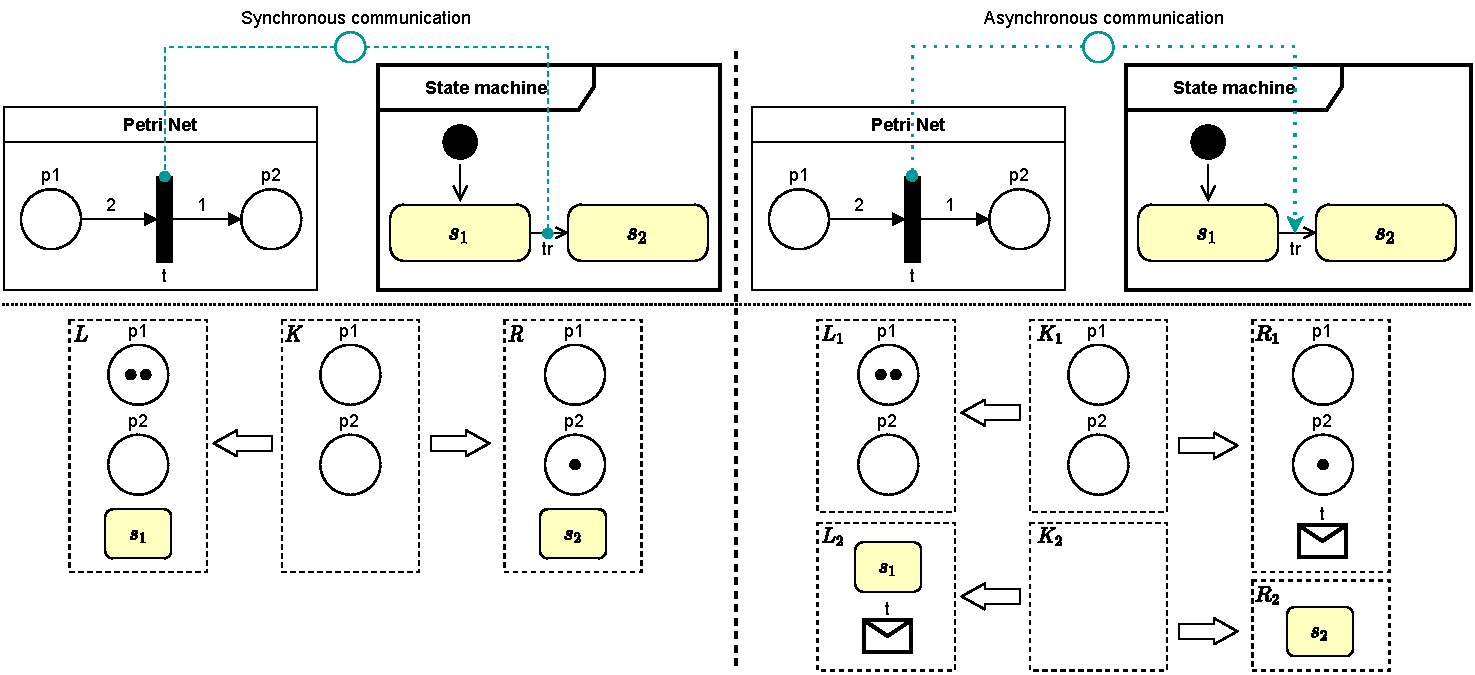
\includegraphics[width=0.95\textwidth]{images/synch_asynch.pdf}
    \caption{\gls*{gg} rules for synchronous and asynchronous interactions}
    \label{fig:synchAsynchInteractions}
\end{figure}

An example of a rule created by synchronous communication can be seen on the left of \autoref{fig:synchAsynchInteractions}.
It shows two pairs of a Petri net and state machine model with one transition each.
The transitions are connected by synchronous communication on the left side and asynchronous communication on the right side (cyan lines).
The lower part of \autoref{fig:synchAsynchInteractions} shows the corresponding \gls*{gg} rules according to our approach.
Synchronous rules can have two or more participants from distinct behavioral models. 

Asynchronous communication will lead to rules being enriched, not merged.
In its simplest form, an asynchronous interaction is directional between two model elements.
It will lead to the creation and consumption of a unique message node.
An example can be seen on the right of \autoref{fig:synchAsynchInteractions}. 
One could also think about asynchronous messages from one model to a set of models, creating multiple messages instead of only one message.
Asynchronous communication influences the global system behavior by forcing two previously unrelated rules to be executed in a particular order.

In addition, we are working towards including a structural model into our approach, which describes how many instances of each behavioral model exist and which of these instances are communicating with whom.
This is useful because we do not want to duplicate behavioral models only to model two instances in our system.
For example, if we have a state machine representing that a resource is acquired or not acquired, we do not want to duplicate this model for every resource in our system.
However, including a structural model makes rule generation more complex since the objects representing instances of behavioral models have to be taken into account.

As a simple example, we want to show how we can use our approach to implement the hierarchical composition of two behavioral models.
Often one wants to specify the behavior of one part of a model in more detail using a separate sub-model.

In \autoref{fig:useCase}, we have a state machine and a \gls*{bpmn} process model where the behavior of the state \texttt{Processing} is described by a \gls*{bpmn} process model.
When the state \texttt{Processing} is entered, a \gls*{bpmn} process should be started, and the state can only be exited when this process is finished.
We can achieve this by synchronizing transition \textit{b} with the \textit{start event} and transition \textit{c} with the \textit{end event} in the \gls*{bpmn} process model, as highlighted by the cyan connections in \autoref{fig:useCase}.

\begin{figure}[h]
    \centering
    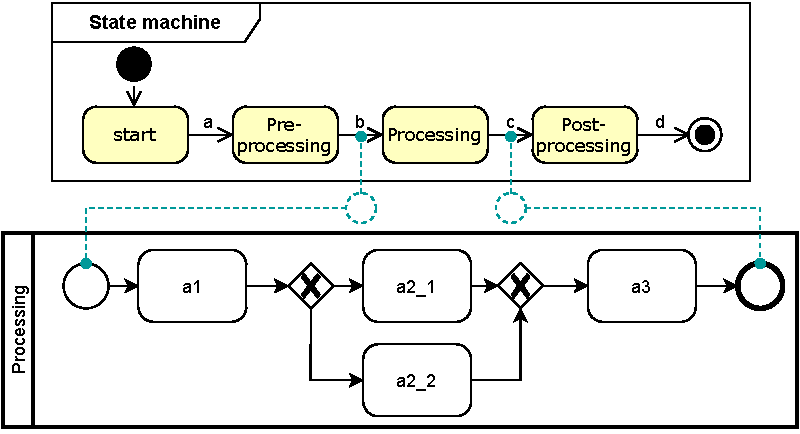
\includegraphics[width=.5\textwidth]{images/usecase.pdf}
    \caption{Hierarchical composition of a state machine and a \gls*{bpmn} process model}
    \label{fig:useCase}
\end{figure}
We implemented the hierarchical composition example in Groove\footnote{\url{https://github.com/timKraeuter/NWPT-2021/tree/main/groove}}.
Groove is a toolset that supports creating and executing \glspl*{gg}, among other things \cite{ghamarianModellingAnalysisUsing2012, rensinkGROOVESimulatorTool2004}.
We manually constructed the \gls*{gg}, which describes the behavior of the composite system, and executed it to check validity.

Using Groove, we can generate the state space of the given \gls*{gg}.
Since the \gls*{gg} describes the composite systems, we can use its state space to check global properties, for example, specified in temporal logic.
The atomic propositions for each state in the global state space can be taken from the individual models because each global state determines which state an individual model has.
We can also analyze the execution path of the individual systems, which is constrained by interactions between them.

\bibliographystyle{plain}
%\bibliographystyle{alpha}
%\bibliographystyle{unsrt}
%\bibliographystyle{abbrv}
\bibliography{bib}

%------------------------------------------------------------------------------
% Index
%\printindex

%------------------------------------------------------------------------------
\end{document}

